Khi ngôn ngữ chung ở dịch vụ máy chủ mở được các nhóm phát triển trong bối cảnh bị giới hạn hạ lưu chấp nhận. Ngôn ngữ chung này được gọi là ngôn ngữ được xuất bản (Published Language). Ngôn ngữ được xuất bản có lợi ích là tính thống nhất trong hệ thống tuy nhiên cần phân tích kĩ vì nó có thể tạo ra sự nhầm lẫn trong bối cảnh bị giới hạn hạ lưu nào đó.

Trong bản đồ bối cảnh, ngôn ngữ được xuất bản kết hợp dịch vụ máy chủ mở được ký hiệu là OHS|PL.

% Vẽ lại bản đồ tiếng Việt

% Vẽ lại bản đồ tiếng Việt

% Vẽ lại bản đồ tiếng Việt

% Vẽ lại bản đồ tiếng Việt

% Vẽ lại bản đồ tiếng Việt

% Vẽ lại bản đồ tiếng Việt

% Vẽ lại bản đồ tiếng Việt

% Vẽ lại bản đồ tiếng Việt

% Từ bản đồ lấy vi dụ cho các mô hình

% Từ bản đồ lấy vi dụ cho các mô hình

% Từ bản đồ lấy vi dụ cho các mô hình

% Từ bản đồ lấy vi dụ cho các mô hình

% Từ bản đồ lấy vi dụ cho các mô hình

% Từ bản đồ lấy vi dụ cho các mô hình

% Từ bản đồ lấy vi dụ cho các mô hình

% Từ bản đồ lấy vi dụ cho các mô hình

% Từ bản đồ lấy vi dụ cho các mô hình

% Từ bản đồ lấy vi dụ cho các mô hình

\begin{example} Trong miền vấn đề ngân hàng, thẻ tín dụng và khoản vay mua nhà không có mối quan hệ.

\begin{figure}[H]

\centering

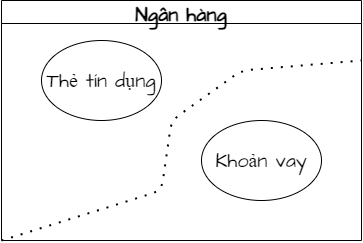
\includegraphics[scale = 0.5]{pictures/mo_hinh_rieng_biet_separate_ways/main.drawio.png}

\caption{Ví dụ mô hình riêng biệt (Separate Ways)}

\end{figure}

\end{example}

